%!TeX root=../pridetop.tex
\chapter[Chapter \thechapter]{}

\begin{figure}[t!]
\centering
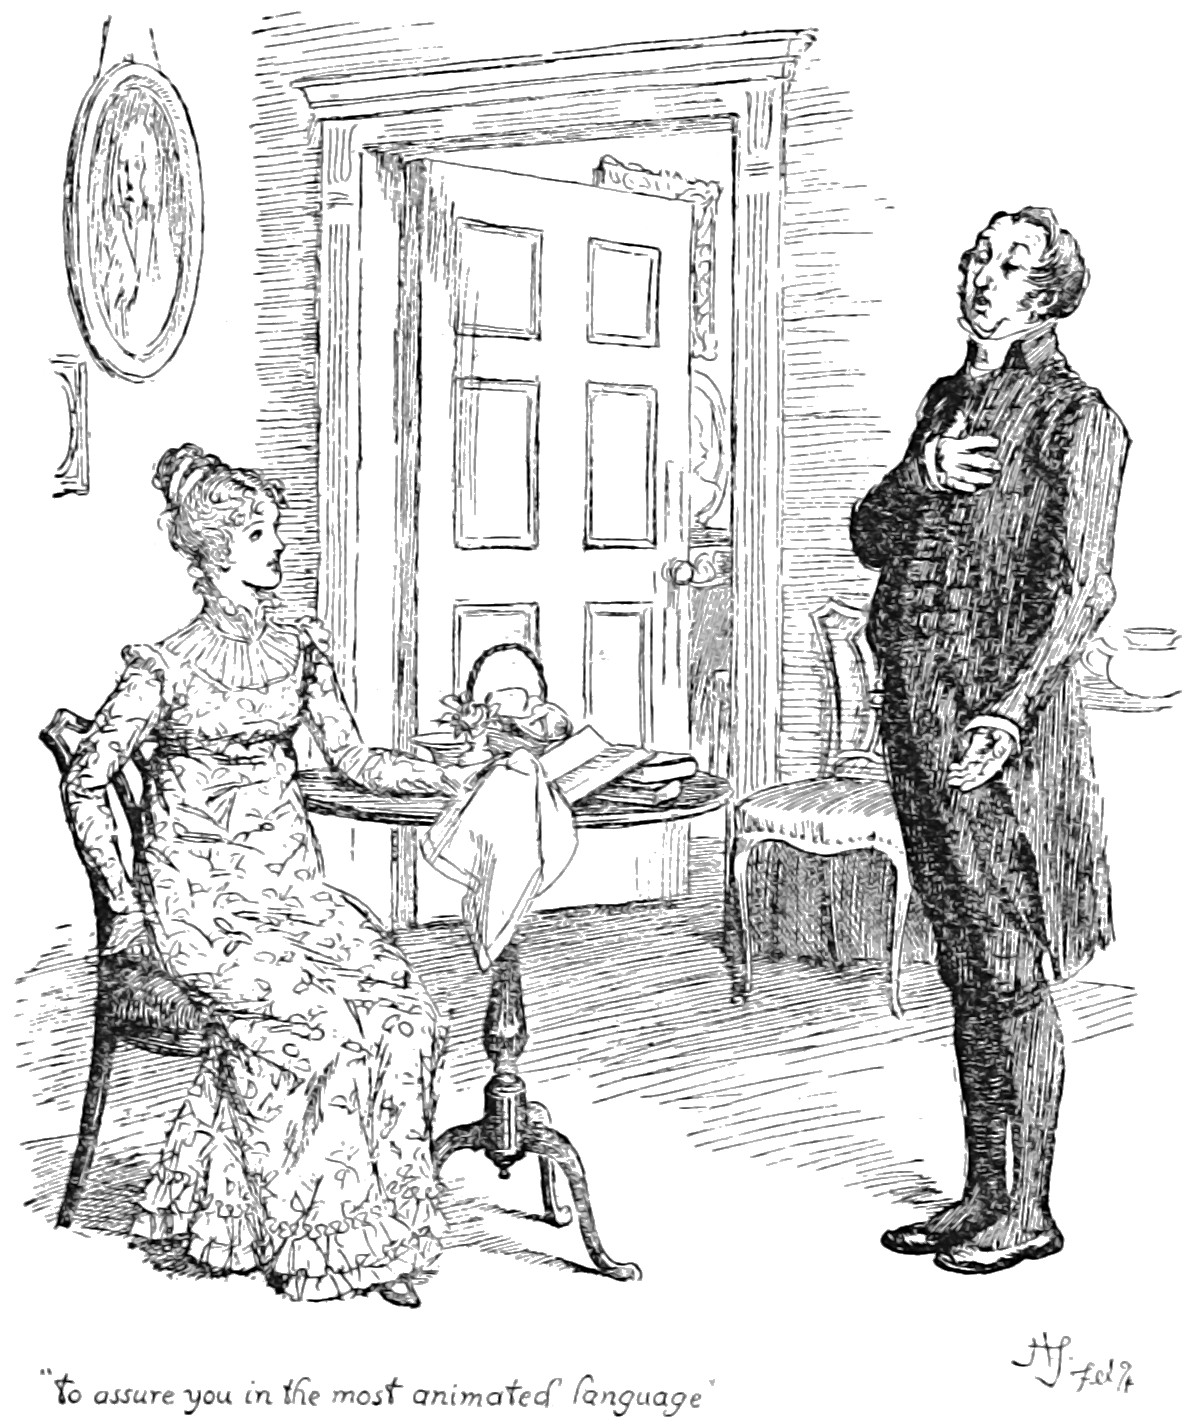
\includegraphics[width=.8\linewidth]{19animated}
\captionlistentry{»To assure you in the most animated language«}
\end{figure}

\lettrine[lines=6,image=true]{initials/chap19t}{he}  next day opened a new scene at Longbourn. Mr Collins made his declaration in form. Having resolved to do it without loss of time, as his leave of absence extended only to the following Saturday, and having no feelings of diffidence to make it distressing to himself even at the moment, he set about it in a very orderly manner, with all the observances which he supposed a regular part of the business. On finding Mrs Bennet, Elizabeth, and one of the younger girls together, soon after breakfast, he addressed the mother in these words,—

»May I hope, madam, for your interest with your fair daughter Elizabeth, when I solicit for the honour of a private audience with her in the course of this morning?«

Before Elizabeth had time for anything but a blush of surprise, Mrs Bennet instantly answered,—

»Oh dear! Yes, certainly. I am sure Lizzy will be very happy—I am sure she can have no objection. Come, Kitty, I want you upstairs.« And gathering her work together, she was hastening away, when Elizabeth called out,—

»Dear ma'am, do not go. I beg you will not go. Mr Collins must excuse me. He can have nothing to say to me that anybody need not hear. I am going away myself.«

»No, no, nonsense, Lizzy. I desire you will stay where you are.« And upon Elizabeth's seeming really, with vexed and embarrassed looks, about to escape, she added, »Lizzy, I \textit{insist} upon your staying and hearing Mr Collins.«

Elizabeth would not oppose such an injunction; and a moment's consideration making her also sensible that it would be wisest to get it over as soon and as quietly as possible, she sat down again, and tried to conceal, by incessant employment, the feelings which were divided between distress and diversion. Mrs Bennet and Kitty walked off, and as soon as they were gone, Mr Collins began,—

»Believe me, my dear Miss Elizabeth, that your modesty, so far from doing you any disservice, rather adds to your other perfections. You would have been less amiable in my eyes had there \textit{not} been this little unwillingness; but allow me to assure you that I have your respected mother's permission for this address. You can hardly doubt the purport of my discourse, however your natural delicacy may lead you to dissemble; my attentions have been too marked to be mistaken. Almost as soon as I entered the house I singled you out as the companion of my future life. But before I am run away with by my feelings on this subject, perhaps it will be advisable for me to state my reasons for marrying—and, moreover, for coming into Hertfordshire with the design of selecting a wife, as I certainly did.«



The idea of Mr Collins, with all his solemn composure, being run away with by his feelings, made Elizabeth so near laughing that she could not use the short pause he allowed in any attempt to stop him farther, and he continued,—

»My reasons for marrying are, first, that I think it a right thing for every clergyman in easy circumstances (like myself) to set the example of matrimony in his parish; secondly, that I am convinced it will add very greatly to my happiness; and, thirdly, which perhaps I ought to have mentioned earlier, that it is the particular advice and recommendation of the very noble lady whom I have the honour of calling patroness. Twice has she condescended to give me her opinion (unasked too!) on this subject; and it was but the very Saturday night before I left Hunsford,—between our pools at quadrille, while Mrs Jenkinson was arranging Miss de Bourgh's footstool,—that she said, »Mr Collins, you must marry. A clergyman like you must marry. Choose properly, choose a gentlewoman for \textit{my} sake, and for your \textit{own}; let her be an active, useful sort of person, not brought up high, but able to make a small income go a good way. This is my advice. Find such a woman as soon as you can, bring her to Hunsford, and I will visit her.« Allow me, by the way, to observe, my fair cousin, that I do not reckon the notice and kindness of Lady Catherine de Bourgh as among the least of the advantages in my power to offer. You will find her manners beyond anything I can describe; and your wit and vivacity, I think, must be acceptable to her, especially when tempered with the silence and respect which her rank will inevitably excite. Thus much for my general intention in favour of matrimony; it remains to be told why my views were directed to Longbourn instead of my own neighbourhood, where I assure you there are many amiable young women. But the fact is, that being, as I am, to inherit this estate after the death of your honoured father (who, however, may live many years longer), I could not satisfy myself without resolving to choose a wife from among his daughters, that the loss to them might be as little as possible when the melancholy event takes place—which, however, as I have already said, may not be for several years. This has been my motive, my fair cousin, and I flatter myself it will not sink me in your esteem. And now nothing remains for me but to assure you in the most animated language of the violence of my affection. To fortune I am perfectly indifferent, and shall make no demand of that nature on your father, since I am well aware that it could not be complied with; and that one thousand pounds in the 4 per cents., which will not be yours till after your mother's decease, is all that you may ever be entitled to. On that head, therefore, I shall be uniformly silent: and you may assure yourself that no ungenerous reproach shall ever pass my lips when we are married.«

It was absolutely necessary to interrupt him now.

»You are too hasty, sir,« she cried. »You forget that I have made no answer. Let me do it without further loss of time. Accept my thanks for the compliment you are paying me. I am very sensible of the honour of your proposals, but it is impossible for me to do otherwise than decline them.«

»I am not now to learn,« replied Mr Collins, with a formal wave of the hand, »that it is usual with young ladies to reject the addresses of the man whom they secretly mean to accept, when he first applies for their favour; and that sometimes the refusal is repeated a second or even a third time. I am, therefore, by no means discouraged by what you have just said, and shall hope to lead you to the altar ere long.«

»Upon my word, sir,« cried Elizabeth, »your hope is rather an extraordinary one after my declaration. I do assure you that I am not one of those young ladies (if such young ladies there are) who are so daring as to risk their happiness on the chance of being asked a second time. I am perfectly serious in my refusal. You could not make \textit{me} happy, and I am convinced that I am the last woman in the world who would make \textit{you} so. Nay, were your friend Lady Catherine to know me, I am persuaded she would find me in every respect ill qualified for the situation.«

»Were it certain that Lady Catherine would think so,« said Mr Collins, very gravely—»but I cannot imagine that her Ladyship would at all disapprove of you. And you may be certain that when I have the honour of seeing her again I shall speak in the highest terms of your modesty, economy, and other amiable qualifications.«

»Indeed, Mr Collins, all praise of me will be unnecessary. You must give me leave to judge for myself, and pay me the compliment of believing what I say. I wish you very happy and very rich, and by refusing your hand, do all in my power to prevent your being otherwise. In making me the offer, you must have satisfied the delicacy of your feelings with regard to my family, and may take possession of Longbourn estate whenever it falls, without any self-reproach. This matter may be considered, therefore, as finally settled.« And rising as she thus spoke, she would have quitted the room, had not Mr Collins thus addressed her,—

»When I do myself the honour of speaking to you next on the subject, I shall hope to receive a more favourable answer than you have now given me; though I am far from accusing you of cruelty at present, because I know it to be the established custom of your sex to reject a man on the first application, and, perhaps, you have even now said as much to encourage my suit as would be consistent with the true delicacy of the female character.«

»Really, Mr Collins,« cried Elizabeth, with some warmth, »you puzzle me exceedingly. If what I have hitherto said can appear to you in the form of encouragement, I know not how to express my refusal in such a way as may convince you of its being one.«

»You must give me leave to flatter myself, my dear cousin, that your refusal of my addresses are merely words of course. My reasons for believing it are briefly these:—It does not appear to me that my hand is unworthy your acceptance, or that the establishment I can offer would be any other than highly desirable. My situation in life, my connections with the family of de Bourgh, and my relationship to your own, are circumstances highly in my favour; and you should take it into further consideration that, in spite of your manifold attractions, it is by no means certain that another offer of marriage may ever be made you. Your portion is unhappily so small, that it will in all likelihood undo the effects of your loveliness and amiable qualifications. As I must, therefore, conclude that you are not serious in your rejection of me, I shall choose to attribute it to your wish of increasing my love by suspense, according to the usual practice of elegant females.«

»I do assure you, sir, that I have no pretensions whatever to that kind of elegance which consists in tormenting a respectable man. I would rather be paid the compliment of being believed sincere. I thank you again and again for the honour you have done me in your proposals, but to accept them is absolutely impossible. My feelings in every respect forbid it. Can I speak plainer? Do not consider me now as an elegant female intending to plague you, but as a rational creature speaking the truth from her heart.«

»You are uniformly charming!« cried he, with an air of awkward gallantry; »and I am persuaded that, when sanctioned by the express authority of both your excellent parents, my proposals will not fail of being acceptable.«

To such perseverance in wilful self-deception Elizabeth would make no reply, and immediately and in silence withdrew; determined, that if he persisted in considering her repeated refusals as flattering encouragement, to apply to her father, whose negative might be uttered in such a manner as must be decisive, and whose behaviour at least could not be mistaken for the affectation and coquetry of an elegant female.
